\chapter{固体物理专题：三维声子、输运与磁性}

\begin{prereqbox}
已经完成晶格、倒格子、单原子链、自由电子气和 Bloch 定理的基础推导。本章补足三维晶格动力学、Kronig--Penney、态密度奇点、Boltzmann 输运和固体磁响应。
\end{prereqbox}
\begin{mapbox}
\[
\begin{aligned}
\text{晶体对称性}&\to\text{允许的 Bloch 态与简并},\\
\text{色散}&\to\text{速度、态密度、响应},
\text{散射机制}&\to\tau,\\
\tau&\to\text{电导、Hall、热导},\\
\text{电子统计}&\to\text{磁性与低温热力学}.
\end{aligned}
\]
\end{mapbox}

\section{点群、空间群与对称性标签}
Bravais 格子描述平移，点群描述保持某点不动的旋转、反射与反演，空间群把二者以及螺旋轴、滑移面统一起来。面试不要求背完 230 个空间群，但要理解三件事：
\begin{enumerate}
\item 对称操作与 Hamiltonian 对易，能态可按不可约表示分类；
\item 高对称 $\vb k$ 点的小群更大，因而常出现受保护简并；
\item 破坏某个对称性会允许原先禁阻的耦合，进而劈裂能级或打开能隙。
\end{enumerate}
若有反演 $P$ 与时间反演 $\Theta$，自旋 $1/2$ 系统中
$P\Theta$ 保持 $\vb k$ 不变且 $(P\Theta)^2=-1$，所以每个 $\vb k$ 上都至少二重简并。若破坏反演但保留时间反演，只有时间反演不变动量处必然 Kramers 简并，其他 $\vb k$ 可发生 Rashba 型分裂。

\section{Kronig--Penney 模型：能带如何整体出现}
考虑周期为 $a$ 的一维 $\delta$ 势
\[
V(x)=P\sum_n\delta(x-na).
\]
单胞内为自由解。用转移矩阵把波函数与导数从一个单胞左侧传到下一个；Bloch 条件要求转移矩阵本征值为 $e^{\pm ika}$。计算迹得到
\[
\boxed{\cos ka=\cos qa+\frac{mP}{\hbar^2q}\sin qa},
\qquad E=\frac{\hbar^2q^2}{2m}.
\]
左边必须落在 $[-1,1]$，因此右边落在区间外的能量不允许，形成禁带。弱势时禁带在自由电子 Bragg 点附近很窄；强势时允许带变窄并接近孤立原子能级展宽。

\begin{whybox}
二能级近自由电子推导解释“某个区边界为什么开隙”，Kronig--Penney 则展示“周期势为什么产生一系列允许带和禁带”。两者是局部与整体视角，不是竞争模型。
\end{whybox}

\section{紧束缚、成键与轨道杂化}
以局域轨道 $|\phi_{n\alpha}\rangle$ 为基，Bloch 和为
\[
|\alpha\vb k\rangle=\frac1{\sqrt N}\sum_n
e^{i\vb k\cdot\vb R_n}|\phi_{n\alpha}\rangle.
\]
Hamiltonian 化为轨道空间矩阵 $H_{\alpha\beta}(\vb k)$。对两个轨道
\[
H(\vb k)=\begin{pmatrix}\epsilon_A&f(\vb k)\\
f^*(\vb k)&\epsilon_B\end{pmatrix},
\]
本征值
\[
E_\pm=\frac{\epsilon_A+\epsilon_B}{2}\pm
\sqrt{\left(\frac{\epsilon_A-\epsilon_B}{2}\right)^2+|f|^2}.
\]
避免交叉的尺度由杂化 $|f|$ 控制；只有当对称性使矩阵元严格为零时，能带交叉才可受保护。

\begin{figure}[htbp]
\centering
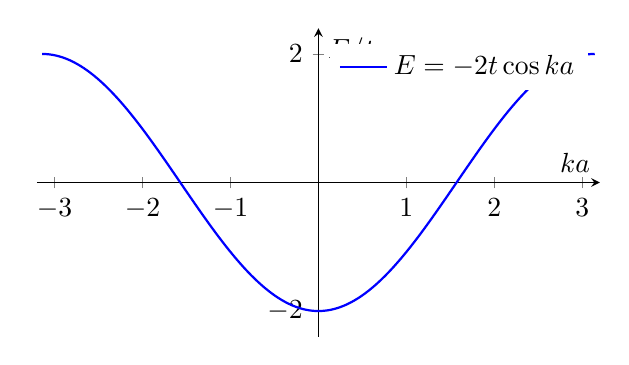
\begin{tikzpicture}
\begin{axis}[width=0.72\textwidth,height=5.5cm,
xlabel={$ka$},ylabel={$E/t$},xmin=-3.2,xmax=3.2,ymin=-2.4,ymax=2.4,
axis lines=middle,samples=160,legend style={draw=none,at={(0.98,0.95)},anchor=north east}]
\addplot[blue,thick,domain=-3.1416:3.1416] {-2*cos(deg(x))};
\addlegendentry{$E=-2t\cos ka$}
\end{axis}
\end{tikzpicture}
\caption{一维最近邻紧束缚能带。带底与带顶曲率符号相反，因而有效质量符号不同。}
\end{figure}

\begin{examplebox}
\textbf{一维二聚化链。}胞内、胞间跃迁为 $t_1,t_2$，
\[
H(k)=\begin{pmatrix}0&t_1+t_2e^{-ika}\\
t_1+t_2e^{ika}&0\end{pmatrix},
\quad E_\pm=\pm|t_1+t_2e^{ika}|.
\]
在 $k=\pi/a$ 的能隙为 $2|t_1-t_2|$。当 $t_1=t_2$，二聚化消失且能隙关闭；这既是 Peierls 图像，也是 SSH 拓扑转变的起点。
\end{examplebox}

\section{态密度与 Van Hove 奇点}
一般能带的态密度
\[
g(E)=\sum_n\int_{\rm BZ}\frac{V\dd^dk}{(2\pi)^d}
\delta[E-E_n(\vb k)].
\]
利用 $\delta$ 函数换元可写为等能面积分
\[
\boxed{g(E)=\sum_n\frac{V}{(2\pi)^d}
\int_{E_n(\vb k)=E}\frac{\dd S}{|\nabla_{\vb k}E_n|}}.
\]
当群速度 $\nabla_kE$ 在极值或鞍点为零时，态密度出现 Van Hove 奇性。一维抛物线带边
$g(E)\propto(E-E_c)^{-1/2}$ 发散；二维抛物线为常数；三维为
$\sqrt{E-E_c}$。二维鞍点常给对数发散，可增强密度波、磁性或超导不稳定性。

\section{三维晶格动力学}
令原胞 $l$ 中第 $\kappa$ 个原子位移为 $u_\alpha(l\kappa)$，谐近似势能
\[
V=\frac12\sum_{l\kappa\alpha,l'\kappa'\beta}
\Phi_{\alpha\beta}(l\kappa,l'\kappa')
u_\alpha(l\kappa)u_\beta(l'\kappa').
\]
代入平面波
\[
u_\alpha(l\kappa,t)=\frac{e_{\kappa\alpha}(\vb q)}
{\sqrt{M_\kappa}}e^{i(\vb q\cdot\vb R_l-\omega t)}
\]
得到动力学矩阵本征问题
\[
\sum_{\kappa'\beta}D_{\kappa\alpha,\kappa'\beta}(\vb q)
e_{\kappa'\beta}=\omega^2(\vb q)e_{\kappa\alpha},
\]
\[
D_{\kappa\alpha,\kappa'\beta}(\vb q)=
\frac1{\sqrt{M_\kappa M_{\kappa'}}}
\sum_{l'}\Phi_{\alpha\beta}(0\kappa,l'\kappa')
e^{i\vb q\cdot(\vb R_{l'}-\vb R_0)}.
\]
每个含 $r$ 个原子的三维原胞有 $3r$ 支：三条声学支和 $3r-3$ 条光学支。声学和规则来自均匀平移不改变能量，保证 $\vb q=0$ 有三个零频模。

量子化位移为
\[
\vb u(l\kappa)=\frac1{\sqrt N}\sum_{\vb q s}
\sqrt{\frac{\hbar}{2M_\kappa\omega_{\vb q s}}}
\vb e_{\kappa s}(\vb q)
(a_{\vb q s}+a_{-\vb q s}^\dagger)
e^{i\vb q\cdot\vb R_l}.
\]
偏振矢量说明原胞内各原子的相对运动，散射实验强度不仅取决于 $\omega$，还取决于偏振与原子散射长度。

\section{电子--声子耦合与电阻温度依赖}
离子位移调制电子周期势，最低阶耦合写成
\[
H_{e-ph}=\sum_{\vb k\vb q s}g_{\vb q s}
c_{\vb k+\vb q}^\dagger c_{\vb k}
(a_{\vb q s}+a_{-\vb q s}^\dagger).
\]
它允许电子吸收或发射声子并改变晶体动量。高温 $T\gtrsim\Theta_D$ 时声子数约正比于 $T$，金属电阻常近似线性；低温只剩小 $q$ 声子，输运还额外抑制小角散射，三维洁净金属出现 Bloch--Grüneisen
$\rho\propto T^5$。杂质给近似温度无关的残余电阻。

\begin{pitfallbox}
Matthiessen 规则 $\rho\simeq\rho_0+\rho_{ph}$ 是独立散射、单一能带等近似下的经验加和，并非严格定理。强各向异性、多带或相干散射时可能失效。
\end{pitfallbox}

\section{Boltzmann 方程与弛豫时间近似}
分布函数 obey
\[
\pdv f t+\dot{\vb r}\cdot\nabla_{\vb r}f
+\dot{\vb k}\cdot\nabla_{\vb k}f
=\left(\pdv f t\right)_{\rm coll}.
\]
均匀稳态、电场作用且
$\hbar\dot{\vb k}=-e\vb E$。取弛豫时间近似
\[
\left(\pdv f t\right)_{\rm coll}=-\frac{f-f_0}{\tau},
\]
令 $f=f_0+\delta f$，保留一阶：
\[
\delta f=e\tau\,\vb E\cdot\vb v
\left(-\pdv{f_0}{E}\right).
\]
电流
\[
j_\alpha=-e\sum_n\int\frac{\dd^3k}{(2\pi)^3}
v_\alpha\delta f
=\sigma_{\alpha\beta}E_\beta,
\]
\[
\boxed{\sigma_{\alpha\beta}=e^2\sum_n\int\frac{\dd^3k}{(2\pi)^3}
\tau_{n\vb k}v_\alpha v_\beta
\left(-\pdv{f_0}{E}\right)}.
\]
$-\partial_Ef_0$ 像宽度 $\kb T$ 的窗口，明确显示输运只取样费米面附近。

\begin{examplebox}
\textbf{恢复 Drude 公式。}各向同性抛物线带中 $\tau$ 为常数，角平均
$\langle v_x^2\rangle=v^2/3$。零温窗口变为
$\delta(E-E_F)$，积分可化为
$\sigma=ne^2\tau/m$。因此 Drude 结果并非只能靠经典碰撞图像，也能由量子统计的 Boltzmann 理论得到。
\end{examplebox}

\section{Hall 效应、多带与磁阻}
有磁场时
\[
\hbar\dot{\vb k}=-e(\vb E+\vb v\times\vb B).
\]
单一各向同性电子带给
$R_H=-1/ne$。若同时有电子和空穴，弱场两带模型
\[
R_H=\frac{p\mu_h^2-n\mu_e^2}
{e(p\mu_h+n\mu_e)^2}.
\]
Hall 符号因此取决于密度和迁移率，不能简单等同于“费米面是电子型还是空穴型”。磁阻反映轨道弯曲、多带补偿、散射各向异性，也可能含弱局域化或自旋散射。

\section{热输运与 Wiedemann--Franz 定律}
温度梯度驱动费米面附近高能粒子从热端向冷端扩散。对弹性散射、简并自由电子，
\[
\kappa=\frac{\pi^2}{3}\frac{n\kb^2T\tau}{m},
\qquad \sigma=\frac{ne^2\tau}{m},
\]
所以
\[
\boxed{\frac{\kappa}{\sigma T}=L_0=
\frac{\pi^2}{3}\left(\frac{\kb}{e}\right)^2}.
\]
这说明热流和电流由相同准粒子承担。强非弹性散射、声子热导、非费米液体或中性激发会使 Lorenz 数偏离 $L_0$。

\section{Pauli 顺磁与 Landau 抗磁}
弱磁场使自旋上下能带相对移动 $\pm\mu_BB$。费米面处转移粒子数约
$g(E_F)\mu_BB$，磁化
\[
M=\mu_B(N_\uparrow-N_\downarrow)
\quad\Rightarrow\quad
\chi_P=\mu_0\mu_B^2g(E_F)
\]
（$g$ 取总态密度时需注意因子约定）。它近似与温度无关，因为只涉及费米面态。

轨道磁场把平面运动量子化成 Landau 能级
\[
E_{n,k_z}=\hbar\omega_c(n+\tfrac12)
+\frac{\hbar^2k_z^2}{2m},
\quad\omega_c=eB/m.
\]
能级随场变化产生抗磁响应。三维自由电子在简单极限下
$\chi_L=-\chi_P/3$。晶体中有效质量、Berry 曲率和多带耦合可显著修改轨道磁性。

\section{量子振荡与费米面}
Landau 能级扫过费米能时，态密度和电阻周期振荡。Onsager 关系
\[
\boxed{F=\frac{\hbar}{2\pi e}A_{\rm ext}},\qquad
\Delta(1/B)=1/F,
\]
把振荡频率 $F$ 与垂直磁场的费米面极值截面积 $A_{\rm ext}$ 相连。温度衰减给回旋有效质量，Dingle 因子给量子寿命，振荡相位可含 Berry 相位信息。

\section{面试总结与自测}
\begin{interviewbox}
\textbf{怎样从一个能带 $E_n(\vb k)$ 推到可观测量？}
先求群速度和曲率；等能面积分给态密度；费米面窗口加散射时间给电导；磁场下半经典轨道或 Landau 量子化给 Hall、磁阻与量子振荡。强调“色散本身还不够，输运还需要占据和散射”。
\end{interviewbox}
\begin{selftestbox}
\begin{enumerate}
\item Kronig--Penney 方程中为何右边超出 $[-1,1]$ 就是禁带？
\item 什么时候两个能带可以真正交叉而非避免交叉？
\item 推导一、二、三维抛物线带边态密度。
\item 三维 $r$ 原子原胞为何有 $3r$ 条声子支？
\item 声学和规则如何约束动力学矩阵？
\item 推导弛豫时间近似下的 $\delta f$。
\item 为什么电导是费米面性质？
\item 两带 Hall 系数为什么可能改变符号？
\item Wiedemann--Franz 定律依赖哪些假设？
\item 量子振荡能测出费米面的哪些信息？
\end{enumerate}
\end{selftestbox}
